% =====================================================================
% CSE 150A Final Project -- DRAFT
% Everything here is a starting point to be rewritten in your own words.
% Lines marked [TODO] need information only the team has.
% Figures are read from ../results/figures/ (they exist on the destin-eval branch).
% =====================================================================
\documentclass[11pt]{article}
\usepackage[margin=1in]{geometry}
\usepackage{graphicx}
\usepackage{booktabs}
\usepackage{amsmath}
\usepackage{amssymb}
\usepackage{hyperref}
\renewcommand{\topfraction}{0.85}
\renewcommand{\textfraction}{0.1}
\renewcommand{\floatpagefraction}{0.75}
\graphicspath{{figures/}{../results/figures/}}

\newcommand{\todo}[1]{\textbf{[TODO: #1]}}

\title{Where Do Wildfires Start? Bayesian Networks for Daily Ignition Risk in San Diego County}
\author{Fire-Fighters \\ Dzaiddin Khazani, Natalin Duangpanya, Alan Jiang, Richard Zamfir, Destin Tanjuaquio}
\date{CSE 150A, Fall 2026}

\begin{document}
\maketitle

\begin{abstract}
We model the daily probability that a wildfire starts in each one-square-mile cell of San Diego
County from weather, terrain, vegetation and the cell's fire history. Using ten years of ignition
records (2015--2024) joined to gridded weather, elevation and vegetation data, we build a
17-million-row cell-day table and compare eight discrete Bayesian network structures, including
hand-built, data-learned (BIC hill climbing) and latent-variable (EM) networks. On held-out years 2023--2024 the learned structure performs best (ROC-AUC
0.829). Conditional independence tests and the structure experiments agree: recent fire history
is by far the strongest signal, temperature adds some information, and humidity, wind and
vegetation add little once these are known.
\end{abstract}

% ---------------------------------------------------------------------
\section{Problem Description}

San Diego County has some of the highest wildfire risk in the United States, and most of its
fires are started by people near roads, homes and the wildland edge. Fire agencies decide where to
patrol, when to issue warnings and where to reduce fuel, and all of these decisions depend on
knowing where and when a fire is likely to start. We ask what the probability is that at least one
fire starts in a given one-square-mile cell on a given day, given the cell's terrain, vegetation
and fire history and the day's weather, and which of these factors still matter once the others
are known.

This is a natural problem for probabilistic reasoning. Ignitions are rare (about 2 per 10,000
cell-days) and noisy, so a model must express uncertainty rather than make hard predictions. The
drivers are also connected to each other: elevation shapes temperature and vegetation, temperature
shapes humidity, and past fires change the vegetation. A Bayesian network lets us write these
relationships down, learn them, query with variables unobserved, and test the assumed dependencies.

Our proposal also planned to compare the model's risk estimates with CAL FIRE's Fire Hazard
Severity Zones (FHSZ). Following our TA's feedback that a direct comparison would be hard to
interpret, we replaced it with a comparison of several network structures, including one with
a latent fire-weather variable learned with EM.

% ---------------------------------------------------------------------
\section{Data Sourcing and Processing}

\textbf{Sources.} Fire ignitions come from the Spatial Wildfire Occurrence Data for the United
States, 1992--2024, 7th edition (FPA-FOD) \cite{fpafod}, about 2.7 million reported wildfires with
discovery date and location (\url{https://doi.org/10.2737/RDS-2013-0009.7}). Daily maximum
temperature, minimum relative humidity and mean wind speed come from gridMET \cite{gridmet}, a
$\sim$4 km grid (\url{https://www.climatologylab.org/gridmet.html}). Vegetation cover and height
come from LANDFIRE 2025 \cite{landfire} 30 m rasters (\url{https://landfire.gov}); vegetation type is
taken from the life-form codes in the cover raster. Elevation and slope come from a USGS digital
elevation model \cite{dem}

\textbf{Building the cell-day table.} We cover the county with 4,678 square cells of 1 mile
(1,609 m) in UTM zone 11N. Each row is one cell on one day, 2015--2024 (17.1 million rows). The
target \texttt{fire} $=1$ if at least one FPA-FOD ignition was discovered in the cell that day.
Elevation is averaged over the cell; slope is computed on a $\sim$30 m grid and then averaged, since
averaging elevation first would flatten the terrain. Vegetation type is the most common life form
in the cell, and cover and height are averaged. Each cell takes the nearest gridMET pixel; coastal
cells whose nearest pixel is ocean are moved to the nearest pixel with data. Fire history
(\texttt{burn\_hist}) is the number of years since the last recorded ignition in the cell, counting
only fires strictly before the current day (back to 1992), so it does not leak the target. It is
ignition history, not burned area.

\textbf{Completeness, missing data and limitations.} We checked every variable in every year. All
4,678 cells appear on all 3,653 days, and weather, elevation and slope have no missing values.
Vegetation is missing for 0.53\% of cell-days, always the same 25 cells on the county edge; none of
the 3,396 fires in 2015--2024 falls in them. Rather than drop these cells we give vegetation an
extra \texttt{missing} state. Fire history is undefined for 45--49\% of cell-days because the cell has
had no fire since 1992; this is information, not missing data, so it gets its own state,
\texttt{none}. The fire records have their own limits: small fires may go unreported, locations are
only accurate to about one cell, and two fires in the same cell on the same day count once. gridMET
pixels are larger than our cells, so neighboring cells often share weather, and daily mean wind
misses short gusts. An early vegetation clip left the north third of the county empty; an input
check caught it and we rebuilt the table.

\textbf{Discretization.} Our networks use discrete conditional probability tables (CPTs), so each
variable is binned into 3--4 states (Table~\ref{tab:bins}, appendix), using fire-weather thresholds
where they exist (minimum humidity below 10\% is critically dry, below 20\% is red-flag range) and
the 2015--2022 distributions elsewhere. Few states matter: a node with $k$ four-state parents has
$4^k$ parent configurations, and we have only a few thousand fires. Vegetation type is collapsed
into non-burnable, shrub and other, since tree and herb cells are each under 4\% of the county.

\textbf{Split and subsampling.} We split by time: 2015--2022 for training (13,669,116 cell-days,
2,861 fires) and 2023--2024 for testing (3,419,618 cell-days, 535 fires). For speed we keep every
training fire but only 2\% of non-fire rows (275,616 rows), each with weight 50. All CPTs are fit
from weighted counts, which are unbiased for the full table, so every CPT describes the real data
and predictions need no correction. The test set is not subsampled.

% ---------------------------------------------------------------------
\section{Modeling and Inference}

\textbf{Algorithms used.} CPTs are learned by maximum likelihood with two smoothed variants;
structures are hand-specified or learned (Chow--Liu for TAN, BIC hill climbing for H); inference
is exact, by variable elimination; and the latent-variable model is learned with EM.

\subsection{Network structures}
All models use the same ten variables. Table~\ref{tab:parents} lists the parents of \texttt{fire} in each structure; Figure~\ref{fig:dags}
shows C and H and Figure~\ref{fig:dags_app} (appendix) the rest.
\begin{itemize}
  \item[A.] \textbf{Naive Bayes:} \texttt{fire} is the parent of every feature, so the features are
  assumed independent given \texttt{fire}. This is the simplest baseline.
  \item[B.] \textbf{TAN:} Naive Bayes plus a tree over the features learned with the Chow--Liu
  algorithm \cite{chowliu,tan}: the maximum spanning tree of the pairwise conditional mutual
  information given \texttt{fire}, oriented away from elevation.
  \item[C.] \textbf{Expert DAG:} 15 edges from domain knowledge. Terrain affects temperature and
  vegetation (elev $\to$ tmax, veg\_type); frequent fire converts shrubland to grass (burn\_hist $\to$
  veg\_type); hot air and strong offshore winds lower humidity (tmax, wind $\to$ rhmin). Wind,
  elevation and vegetation cover and height are left out as parents of \texttt{fire}: we assume
  daily wind drives spread rather than ignition, and the others act through fire's parents.
  \item[D.] \textbf{Expert DAG + latent regime:} a hidden variable \texttt{danger} with $K=2,3,4$
  states becomes a parent of tmax, rhmin, wind and fire, replacing the weather $\to$ fire edges.
  The three weather readings are treated as symptoms of one regime (e.g.\ offshore Santa Ana flow
  vs.\ onshore marine layer), and a shared hidden parent lets wind and temperature depend on each
  other, which C forbids.
  \item[E--G.] \textbf{One-hypothesis variants of C} that change only the parents of \texttt{fire}:
  E (\emph{fuel structure}) asks whether vegetation cover and height add to vegetation type;
  F (\emph{no weather}) removes every weather $\to$ fire edge; G (\emph{fuel + history only}) is
  the leanest ``human ignition'' model. Any score difference from C can be attributed to that change.
  \item[H.] \textbf{Hill climbing:} no hand-picked edges. Starting from an empty graph we greedily
  add, remove or reverse the single edge that most improves the BIC score on the training data,
  keeping the graph acyclic with at most 4 parents per node, until no move helps.
\end{itemize}

\begin{table}[htb]
\centering
\small
\begin{tabular}{llr}
\toprule
Structure & Parents of \texttt{fire} & Rows \\
\midrule
A, B & none (\texttt{fire} is the parent of every feature) & 1 \\
C. Expert & tmax, rhmin, veg\_type, burn\_hist, slope & 1,024 \\
D. Latent & \texttt{danger}, veg\_type, burn\_hist, slope & $64K$ \\
E. Fuel structure & rhmin, veg\_type, veg\_cover, veg\_height, burn\_hist & 1,600 \\
F. No weather & veg\_type, burn\_hist, slope & 64 \\
G. Fuel + history & veg\_type, veg\_cover, veg\_height, burn\_hist & 400 \\
H. Hill climbing & tmax, burn\_hist & 16 \\
\bottomrule
\end{tabular}
\caption{Parents of \texttt{fire} in each structure. C--G share the expert edges among the features (E and G also add veg\_cover $\to$ veg\_height). Rows = parent configurations in fire's CPT.}
\label{tab:parents}
\end{table}

\begin{figure}[htb]
\centering
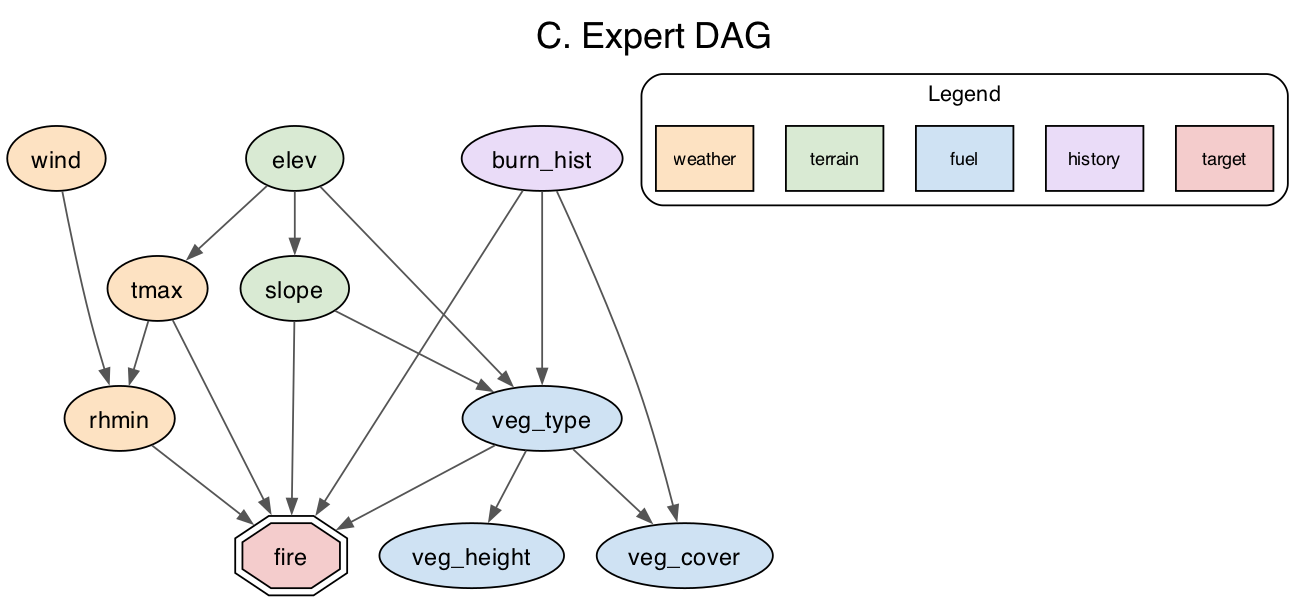
\includegraphics[width=0.49\linewidth]{dag_expert.png}
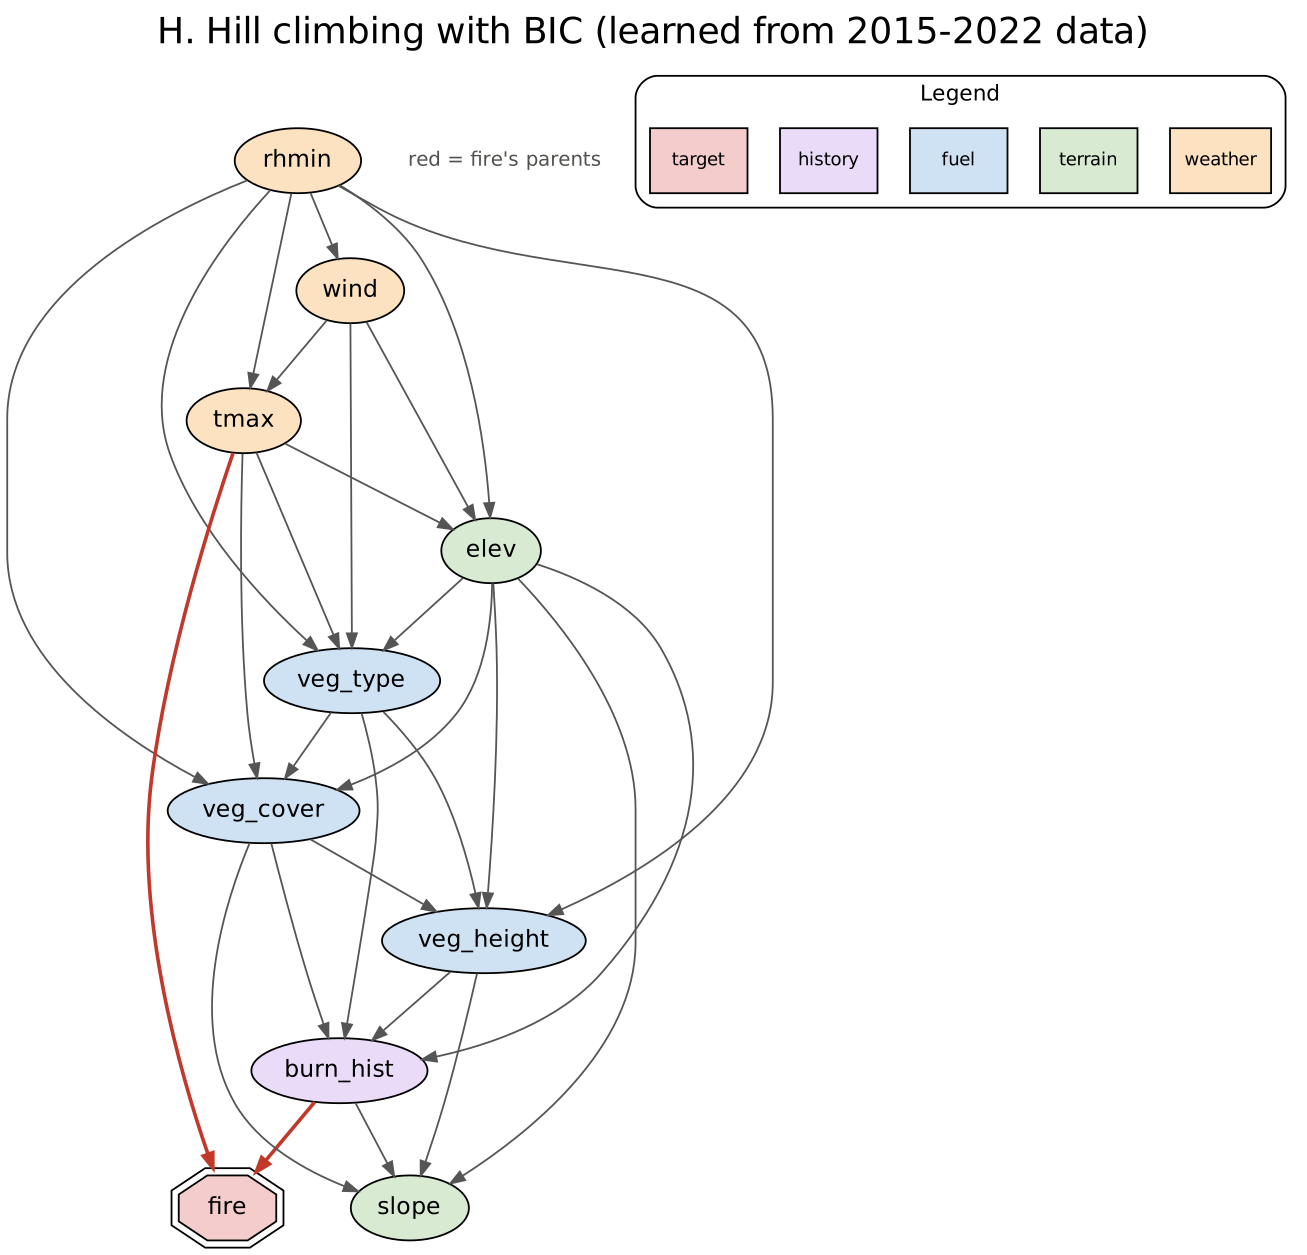
\includegraphics[width=0.40\linewidth]{dag_hillclimb.png}
\caption{(C) Expert DAG and (H) structure learned by BIC hill climbing, with fire's two parents in
red. The other structures, including D with its latent node, are in Figure~\ref{fig:dags_app} (appendix).}
\label{fig:dags}
\end{figure}

\subsection{Parameter learning}
Each CPT is estimated from weighted counts $N(x,\mathrm{pa})$ by MLE, $N(x,\mathrm{pa})/N(\mathrm{pa})$;
by BDeu, which adds $\alpha=\text{ESS}/(rq)$ to every count; or by a Dirichlet prior centred on the
marginal, $\big(N(x,\mathrm{pa}) + \text{ESS}\cdot P(x)\big)/\big(N(\mathrm{pa})+\text{ESS}\big)$, with
equivalent sample size $\text{ESS}=10$ ($r$ states of $x$, $q$ parent configurations). They differ on
parent configurations never seen in training: MLE and BDeu give these a (nearly) uniform row, i.e.\
$P(\text{fire})=0.5$, while the marginal prior falls back to the overall rate, $\approx 0.0002$.

\subsection{Learning the latent model with EM}
\texttt{danger} is never observed, so model D is fit by EM on the weighted training rows. The
E-step computes each row's posterior over the hidden state given all ten observed variables:
\[
q_i(h) \propto P(h)\,P(\text{tmax}_i \mid \text{elev}_i, h)\,P(\text{rhmin}_i \mid \text{tmax}_i, \text{wind}_i, h)\,
P(\text{wind}_i \mid h)\,P(\text{fire}_i \mid \text{pa}_i, h),
\]
since every other factor cancels. The M-step refits these five CPTs from expected counts (row $i$
adds $w_i q_i(h)$ to state $h$) with the marginal Dirichlet prior, so this is MAP-EM. We run several
random initializations, stop at a relative log-likelihood change below $10^{-9}$ or 400 iterations,
and keep the best run. Each cell-day gets its own hidden state; a true weather regime would be shared
by all cells on a day, so D is a per-row mixture rather than a day-level regime.

\subsection{Inference and evaluation}
We implemented exact inference by variable elimination, which multiplies CPT factors and sums out
unobserved variables; it is used for the sanity and diagnostic queries. For test prediction all
features are observed, so $P(\text{fire}\mid\mathbf{x})$ needs only the CPTs that mention
\texttt{fire}; our batched version matches full variable elimination to $10^{-12}$ on 200 random rows.
For D the hidden state is summed out. Baselines are a constant (training fire rate) and a weighted
logistic regression on one-hot features. We report log-loss, Brier score, PR-AUC and ROC-AUC with
95\% intervals from 1,000 bootstrap replicates that resample whole test \emph{days}, because cells on
the same day share weather.

\subsection{Conditional independence tests}
\label{sec:ci}
Since \texttt{fire} has no children in C, the DAG claims $\text{fire}\perp X \mid
\text{parents(fire)}$ for every non-parent $X$; it also claims its root nodes are independent. We
test these with stratified G-tests on the full, unweighted 2015--2022 data. The tables are sparse
(about 1,000 strata, 2,861 fires): under independence $G$ averages 5--15\% below its degrees of
freedom, so for tests involving \texttt{fire} we simulate the null by redrawing the fires within each
stratum (multivariate hypergeometric, 2,000 replicates). Because millions of rows make tiny effects
significant, we also report the bias-corrected conditional mutual information $(G-\mathbb{E}_0[G])/2N$.
The Bonferroni threshold is $0.05/13=0.0038$.

% ---------------------------------------------------------------------
\section{Results and Discussion}
\label{sec:results}

\begin{table}[htb]
\centering
\small
\begin{tabular}{lcccc}
\toprule
Model & Log-loss ($\times10^{-3}$) & Brier ($\times10^{-4}$) & PR-AUC ($\times10^{-4}$) & ROC-AUC \\
\midrule
Constant rate & 1.535 & 1.564 & 1.57 & 0.500 \\
Logistic regression & 1.444 & 1.564 & 8.37 & 0.825 [0.809, 0.841] \\
A. Naive Bayes & 1.446 & 1.565 & 7.53 & 0.815 [0.798, 0.831] \\
B. TAN & 1.480 & 1.568 & 6.72 & 0.814 [0.798, 0.830] \\
C. Expert DAG & 1.428 & 1.564 & 7.73 & 0.814 [0.796, 0.832] \\
D. Latent, $K=3$ & 1.420 & 1.564 & 6.97 & 0.816 [0.799, 0.832] \\
E. Fuel structure & 1.443 & 1.564 & 6.03 & 0.797 [0.779, 0.814] \\
F. No weather & 1.435 & 1.564 & 5.36 & 0.799 [0.783, 0.816] \\
G. Fuel + history & 1.434 & 1.564 & 5.71 & 0.805 [0.788, 0.822] \\
H. Hill climbing & \textbf{1.404} & 1.564 & 7.29 & \textbf{0.829} [0.813, 0.845] \\
\bottomrule
\end{tabular}
\caption{Test results, 2023--2024 (535 fires). All networks use the marginal Dirichlet estimator.
Random PR-AUC $=1.56\times10^{-4}$. Full results with intervals for every structure and estimator:
\texttt{results/metrics.md}, \texttt{results/latent\_em.md}.}
\label{tab:metrics}
\end{table}

\textbf{Structures.} Table~\ref{tab:metrics} gives the test results; differences below are
paired bootstrap 95\% intervals. All networks reach about 5 times the random PR-AUC. The hand-built
expert DAG C beats Naive Bayes on log-loss by $1.9\times10^{-5}$ [$0.3, 3.3$]$\times10^{-5}$, while TAN
is \emph{worse} than Naive Bayes ($+3.4\times10^{-5}$): its tree is chosen to capture dependencies
among the features, not to predict \texttt{fire}. The learned structure H is the best model: it beats C
on log-loss by $2.4\times10^{-5}$ [$1.1, 3.7$]$\times10^{-5}$ and on ROC-AUC by 0.015 [0.005, 0.025],
and edges past logistic regression. It gives \texttt{fire} only two parents, burn\_hist and tmax, so
its fire CPT has 16 well-populated rows instead of C's 1,024. Larger fire tables overfit:
measured as the log-loss improvement over the constant predictor, C gains 9.9\% on training data
but only 6.5\% on test data and E 8.8\% vs.\ 5.5\%, while H's 8.2\% carries over almost fully
(8.1\%). With about 2,900 training fires, C's table averages $\sim$3 fires per row and H's $\sim$180.

\textbf{What the variants show.} F, which drops all weather edges, has the same log-loss as C
(difference not significant) but significantly lower ROC-AUC ($-0.015$) and PR-AUC (by about 30\%): weather,
through temperature, helps \emph{rank} risky days even if it barely changes average accuracy. E, which
swaps temperature and slope for vegetation cover and height, is significantly worse on ROC-AUC
($-0.017$); more detail on fuel does not replace temperature. G (fuel and history only) is similar: significantly lower PR-AUC, with a ROC-AUC difference that is not significant.

\textbf{Estimators.} For A, B and H the three estimators agree to three digits, since every parent
configuration is well populated. For C, 343 of fire's 1,024 parent configurations never occur in
training; MLE and BDeu set these to $P(\text{fire})=0.5$, more than doubling the overall fire rate
(0.00047 vs.\ 0.00021), while the marginal Dirichlet prior restores 0.000217 and the best log-loss.

\textbf{What the models learned.} Fire history dominates: 46\% of training fires occur in cells with
an ignition in the previous two years (10\% of cell-days), and only 6.5\% in cells with no fire since
1992 (48\% of cell-days). Ignitions recur in the same places, as expected if most are started by
people along roads and the wildland--urban edge. Weather is weaker than expected: hot days have the
highest ignition rate, but critically dry, extreme-heat and strong-wind days are \emph{below} average
(Figure~\ref{fig:binrates}, appendix), plausibly because FPA-FOD records ignitions, and extreme
weather mainly makes fires grow. Steep slopes have far fewer ignitions, consistent with human access.
H's fire CPT (Table~\ref{tab:hcpt}, appendix) makes the trade-off concrete: a recent ignition in
the cell raises the daily rate about 30--60 times compared with no fire since 1992, while going
from cool to hot raises it 3--5 times. Only 3.3\% of the county's recorded ignitions have a
natural cause, so fire history most likely stands in for where people are.

\textbf{Testing C's assumptions.} (Table~\ref{tab:ci}, appendix.) Leaving wind out of fire's parents
is supported ($p=0.097$), but elevation and vegetation cover still carry information given the
parents ($p=0.0005$). Among the included parents, fire history is by far the strongest, then
temperature; humidity ($p=0.014$) and vegetation type ($p=0.0075$) are not significant once the
others are known. This agrees with H, which keeps exactly burn\_hist and tmax. The root-node claims
all fail, most strongly wind $\perp$ tmax $\mid$ elev (0.057 nats); H also links wind, temperature and
elevation. These violations do not change test predictions, since $P(\text{fire}\mid\text{all})$
depends only on fire's parents, but they bias queries that sum variables out. p-values are somewhat
optimistic because rows are correlated, so we rely mainly on effect sizes.

\textbf{Latent weather regimes (D).} Training log-likelihood and BIC improve with every added state,
but test log-loss is best at $K=3$ (1.420, vs.\ 1.424 for $K=2$ and 1.421 for $K=4$). D's log-loss is
slightly below C's but the interval includes zero, and its PR-AUC is lower, so it is about as good a
predictor, not a better one. With $K=3$ the states are interpretable (Figure~\ref{fig:months},
appendix): a cool, humid, windy state concentrated in December--March (winter storms; 1.1 fires per
10,000 cell-days), a warm, dry state spread through the year (1.7), and a hot state dominant in
June--September (3.0). No hot-dry-windy ``Santa Ana'' state appears: in daily means strong wind goes
with storms, and Santa Ana days are too rare to earn a state in a per-row mixture.

\textbf{Convergence and scalability.} Models without hidden variables are fit in one pass of weighted
counting (seconds); hill climbing takes 29 moves, and the two edges into \texttt{fire} come near the end with the smallest score gains: the BIC is dominated by dependencies among the features. EM takes
$\sim$0.15 s per iteration. Its log-likelihood rises steeply for about 20 iterations and then
flattens (\texttt{results/figures/em\_convergence.png}); for $K=2$ one of three random starts ended in
a clearly worse local optimum, and for $K=3,4$ runs hit the 400-iteration cap with starts still
disagreeing, so more restarts would help. The limit is data, not computation: CPT size grows as $4^k$ in the number of
parents while we have 2,861 training fires, which is why the sparse structures (H, Naive Bayes) are
the most stable. The learned structure is itself stable: fire's parents are \{burn\_hist, tmax\}
for parent limits of 2--5, for different training years and across 10 bootstrap resamples. Finally, 2023--2024 had fewer fires than the training years (0.00016 vs 0.00021),
so every model over-predicts slightly on the test set (Figure~\ref{fig:calib}, appendix).

% ---------------------------------------------------------------------
\section{Conclusion}
\label{sec:conclusion}
Eight Bayesian network structures predict daily ignitions in San Diego County with ROC-AUC between
0.797 and 0.829. The best is the structure learned by BIC hill climbing, which beats both our
hand-built expert DAG and logistic regression. Three lines of evidence agree on what
matters: the independence tests, the one-change variants E--G, and the learned structure all point to
fire history first and temperature second, with humidity, wind and vegetation adding little once these
are known. This fits ignitions being mostly human-caused. Smoothing toward the marginal is essential
for structures with many parents of \texttt{fire}. A latent weather regime learned by EM finds
interpretable seasonal states but does not improve prediction.

\textbf{Limitations.} We have no direct measure of human activity (roads, population, power
lines), so fire history and terrain stand in for it; fire history is ignition history from point
records, not burned area; rows are correlated in space and time, so tests and intervals are
approximate; and the fire rate shifts between years.

\textbf{Extensions.} A latent regime shared by all cells on a day (an E-step over days), which may
isolate Santa Ana days; more EM restarts for $K\ge3$; road and population data; and the comparison
with CAL FIRE's hazard zones from our proposal.

% ---------------------------------------------------------------------
\section{Reflections and Contributions}

\textbf{Advice for future students: } Start the data pipeline early. The hardest part is getting started so the sooner you have the data the easier it is to work on the rest of the project.

\textbf{Contributions and reflections.}
\begin{itemize}\setlength{\itemsep}{1pt}\setlength{\parskip}{0pt}
  \item \textbf{Dzaiddin Khazani:} I procured data that would be needed to analyze the problem (fire statistics, weather, topography et cetera) specifically to the San Diego County area and built a program to compile all of these information into a workable and analyzable cell-day tables for the algorithms to take as an input. I also helped plan our project's structure and how we can approach the problem statement that we had in mind. I learned a lot about how different kind of algorithms can be used to solve aspects of our larger problem, and how important deciding a concrete solvable problem is for this project.
  \item \textbf{Destin Tanjuaquio:} I fit Naive Bayes, TAN, and an expert DAG and evaluated against baselines with bootstrap confidence intervals.
  \item \textbf{Natalin Duangpanya:} I contributed to the project by plotting each variable's distribution, discretizing the data into bins, splitting the data into training/testing sets, and defining and diagraming the structures for the Naive Bayes, Tree-augmented Naive Bayes, and Expert DAGS. Overall, my understanding of real-world applications of Naive Bayes models has increased after this project. In addition, I have learned that visualizing the data and models is crucial for the data exploration process, helping us set bin edges and better understand the independence assumptions each network makes.
  \item \textbf{Alan Jiang:} I designed different DAG structures. My work is necessary to confidently answer the research question because it gives us additional baseline DAG models that ground our results as real and substantially accurate findings towards the research question.
  \item \textbf{Richard Zamfir}: I reviewed the team's branches, ran conditional independence  tests on the expert DAG, added the latent weather model fit with EM, and assembled and edited the final report. One thing I learned was that EM only guarantees a local optimum. with two hidden states, one of our three random starts converged to a clearly worse solution than the other two, so running several restarts and keeping the best one was necessary.
 \end{itemize}

\textbf{Use of generative AI.}
\begin{itemize}\setlength{\itemsep}{1pt}\setlength{\parskip}{0pt}
  \item \textbf{Dzaiddin Khazani:} I used Generative AI to help plan the structure of this project. I also used it to help write programs to consolidate all of the datasets that we have identified to help in our project.
  \item \textbf{Destin Tanjuaquio:} I used AI to review my approach and suggest/explain concepts before implementation, as well as summarizing current state of project after my work.
  \item \textbf{Natalin Duangpanya:} I used AI to help me reclip the data and rebuild the cell day tables, create an implementation plan for phases 3 and 4 from the given project plan and help me understand how to use libraries such as NetworkX and Graphviz.
  \item \textbf{Alan Jiang:} I utilized AI mainly to summarize committed work to the repository as well as explain certain parts that I was confused about in order to stay up to speed with the project and progress. I also used it to help me in implementing the different model structures, like checking logic/debugging, to allow me to focus more on actually designing different model structures.
  \item \textbf{Richard Zamfir} I used AI to help me collect the work from the repository branches, discuss independence testing and EM code, condense, spell-check, and fix the grammar of the final report.
\end{itemize}


% ---------------------------------------------------------------------
\begin{thebibliography}{9}
\bibitem{fpafod} Short, K.~C. (2026). Spatial wildfire occurrence data for the United States,
1992--2024 [FPA\_FOD\_20260615]. 7th Edition. Fort Collins, CO: Forest Service Research Data
Archive. \url{https://doi.org/10.2737/RDS-2013-0009.7}
\bibitem{gridmet} Abatzoglou, J.~T. (2013). Development of gridded surface meteorological data
for ecological applications and modelling. \emph{International Journal of Climatology}, 33(1), 121--131.
\url{https://www.climatologylab.org/gridmet.html}
\bibitem{landfire} LANDFIRE (2025). Existing Vegetation Type, Cover and Height, LF 2025.
U.S. Department of the Interior, Geological Survey, and U.S. Department of Agriculture.
\url{https://landfire.gov}
\bibitem{dem} U.S. Geological Survey.
\bibitem{tiger} U.S. Census Bureau (2024). TIGER/Line Shapefiles: Counties.
\url{https://www.census.gov/geographies/mapping-files/time-series/geo/tiger-line-file.html}
\bibitem{chowliu} Chow, C. and Liu, C. (1968). Approximating discrete probability distributions
with dependence trees. \emph{IEEE Transactions on Information Theory}, 14(3), 462--467.
\bibitem{tan} Friedman, N., Geiger, D. and Goldszmidt, M. (1997). Bayesian network classifiers.
\emph{Machine Learning}, 29, 131--163.
\bibitem{libs} Python libraries: NumPy, pandas, networkx, scikit-learn, SciPy, rasterio,
geopandas, xarray, matplotlib.
\end{thebibliography}

\appendix
\section{Additional tables and figures}
\label{app:tables}

\begin{table}[htbp]
\centering
\begin{tabular}{lll}
\toprule
Variable & Bin edges & States \\
\midrule
tmax (\textdegree C) & 20, 28, 35 & cool, mild, hot, extreme \\
rhmin (\%) & 10, 20, 35 & crit\_dry, dry, moderate, humid \\
wind (m/s) & 2, 3, 4.5 & calm, light, moderate, strong \\
elev (m) & 200, 600, 1200 & low, foothill, mountain, high \\
slope (\textdegree) & 5, 15, 25 & flat, rolling, steep, very\_steep \\
veg\_type & -- & nonburnable, shrub, other\_veg, missing \\
veg\_cover (\%) & 5, 20, 35 & bare, sparse, moderate, dense, missing \\
veg\_height (m) & 0.5, 1.5, 3 & low, low\_shrub, tall\_shrub, tree, missing \\
burn\_hist (years) & 2, 10 & recent, mid, old, none \\
\bottomrule
\end{tabular}
\caption{Discretization of each variable. Bins are right-open.}
\label{tab:bins}
\end{table}

\begin{table}[htbp]
\centering
\begin{tabular}{lccl}
\toprule
Claim & p & Effect vs.\ slope edge & Verdict \\
\midrule
fire $\perp$ wind $\mid$ parents & 0.097 & 0.57 & holds \\
fire $\perp$ veg\_height $\mid$ parents & 0.004 & 1.16 & holds (borderline) \\
fire $\perp$ elev $\mid$ parents & 0.0005 & 1.97 & rejected \\
fire $\perp$ veg\_cover $\mid$ parents & 0.0005 & 1.39 & rejected \\
\midrule
fire $\perp$ burn\_hist $\mid$ other parents & 0.0005 & 43.1 & edge supported \\
fire $\perp$ tmax $\mid$ other parents & 0.0005 & 7.7 & edge supported \\
fire $\perp$ slope $\mid$ other parents & 0.001 & 1.0 & edge supported \\
fire $\perp$ rhmin $\mid$ other parents & 0.014 & 0.68 & weak \\
fire $\perp$ veg\_type $\mid$ other parents & 0.0075 & 0.77 & weak \\
\midrule
wind $\perp$ tmax $\mid$ elev & $<10^{-300}$ & -- & rejected (0.057 nats) \\
elev $\perp$ burn\_hist (cell-year) & $<10^{-300}$ & -- & rejected (0.023 nats) \\
wind $\perp$ elev & $<10^{-300}$ & -- & rejected (0.014 nats) \\
wind $\perp$ burn\_hist & $<10^{-300}$ & -- & rejected (0.003 nats) \\
\bottomrule
\end{tabular}
\caption{Conditional independence tests on the expert DAG (2015--2022). p-values for fire
tests are Monte Carlo (resolution 0.0005). Effect = bias-corrected conditional mutual
information divided by that of the slope edge. Full table: \texttt{results/independence\_tests\_expert.md}.}
\label{tab:ci}
\end{table}

\begin{figure}[htbp]
\centering
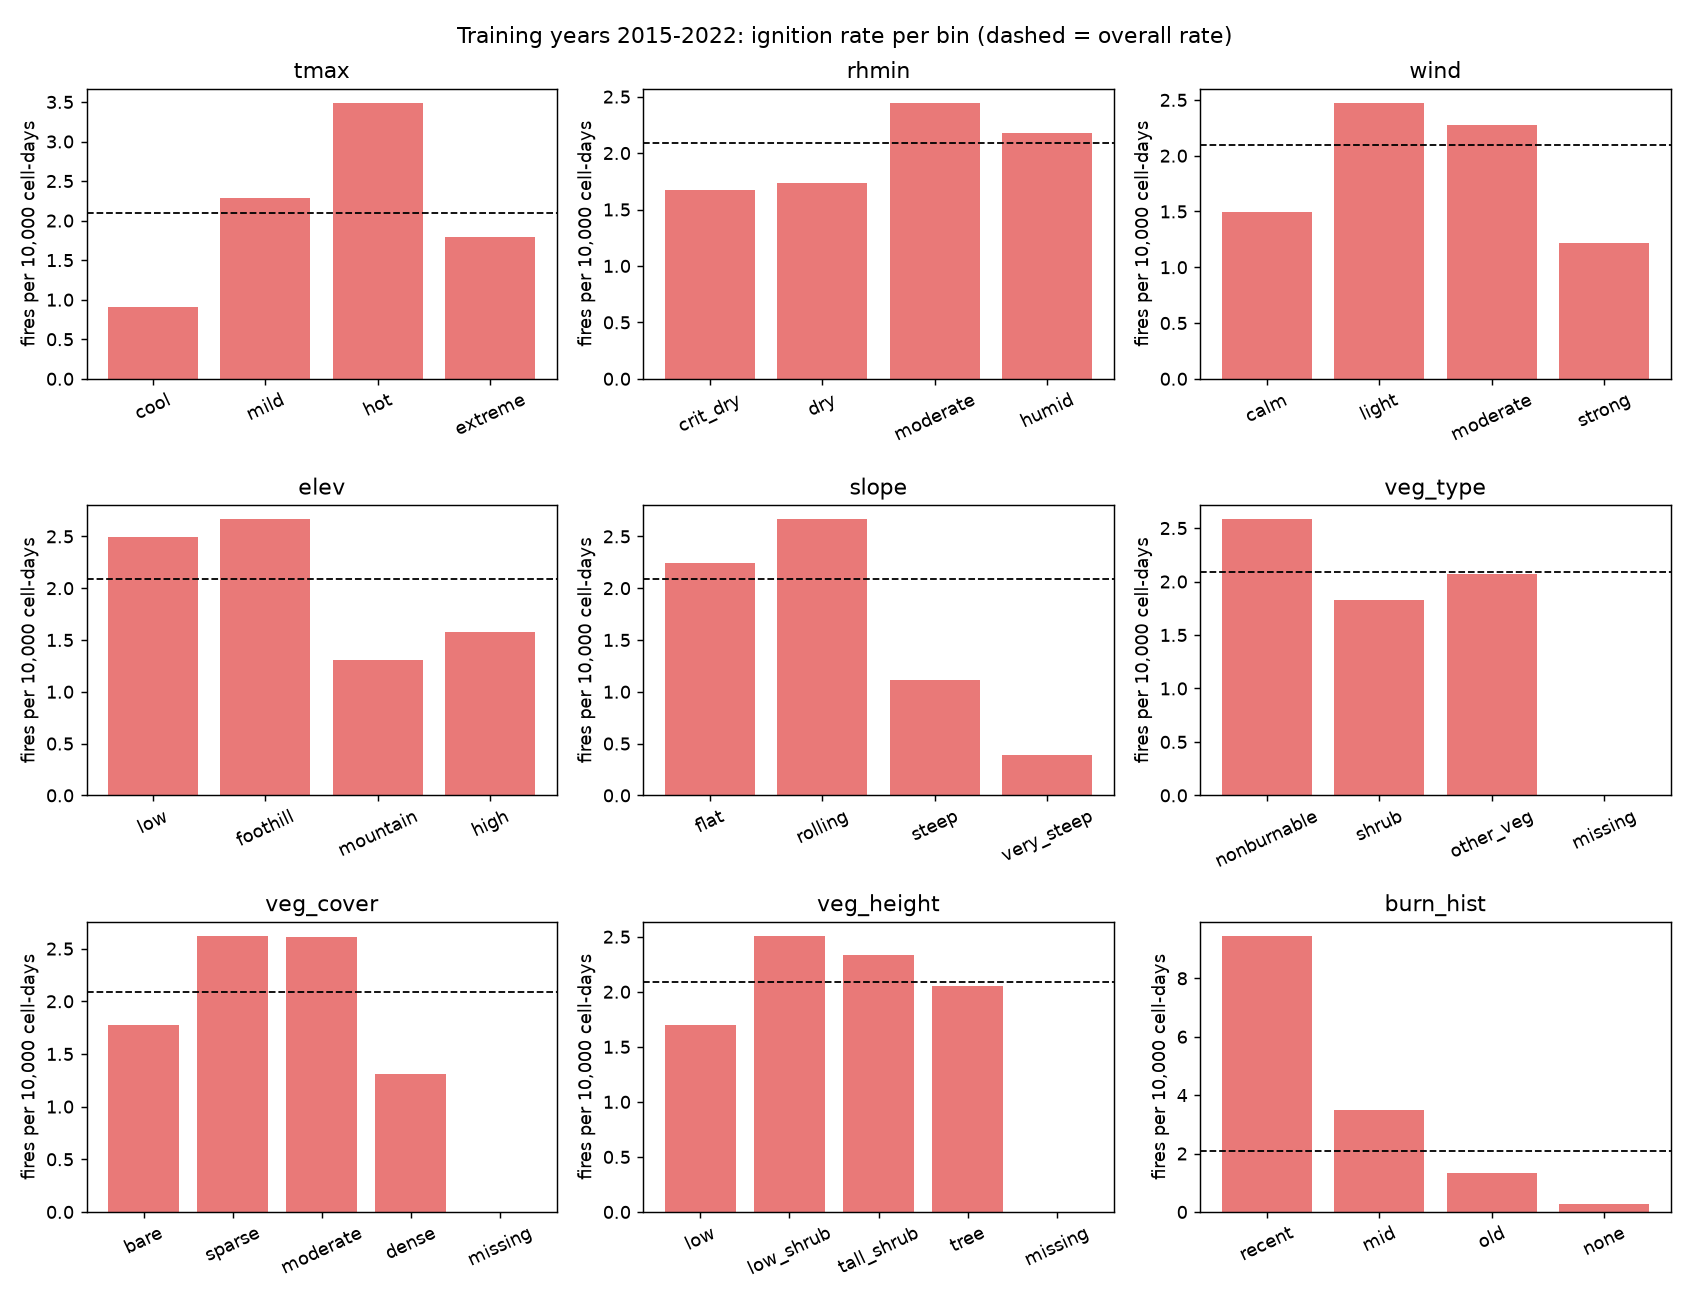
\includegraphics[width=0.85\linewidth]{bin_fire_rates.png}
\caption{Ignitions per 10,000 cell-days in each bin, 2015--2022. Dashed line: overall rate.}
\label{fig:binrates}
\end{figure}

\begin{figure}[htbp]
\centering
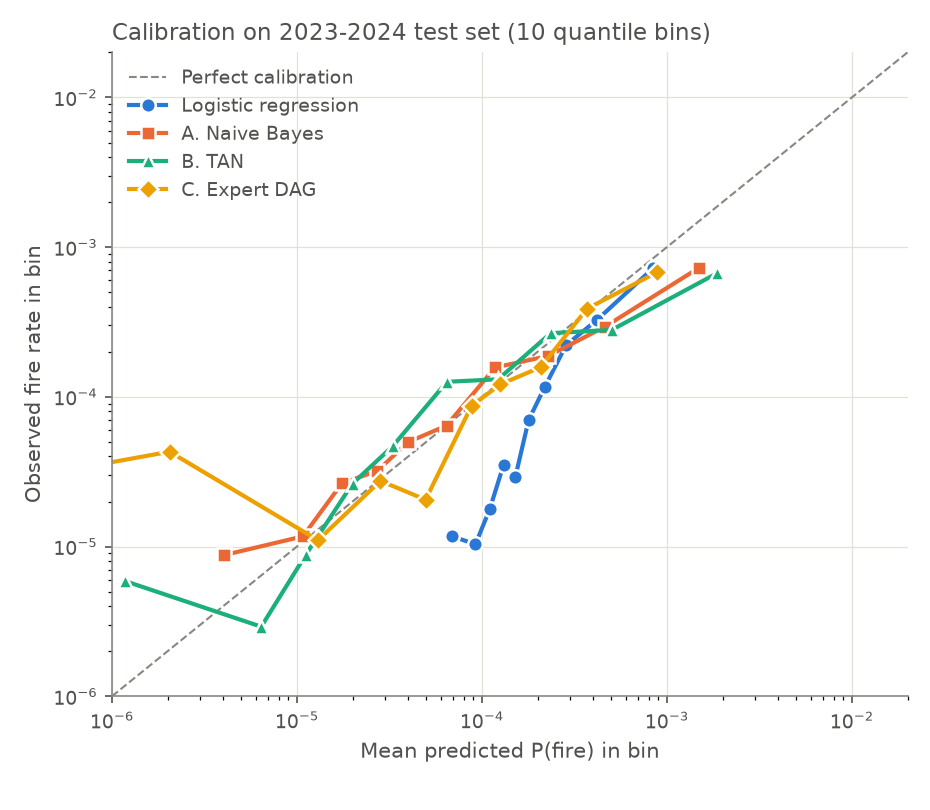
\includegraphics[width=0.5\linewidth]{calibration.png}
\caption{Calibration on 2023--2024 (10 quantile bins of predicted probability).}
\label{fig:calib}
\end{figure}

\begin{figure}[htbp]
\centering
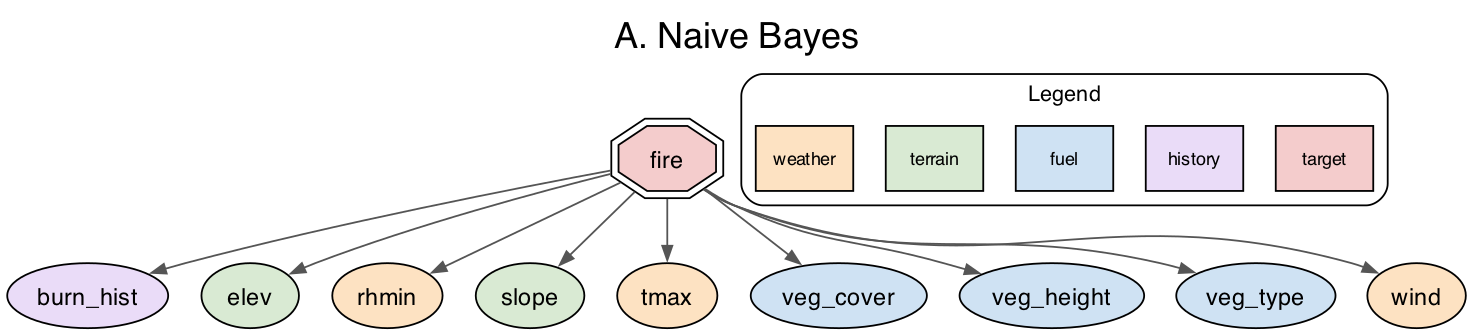
\includegraphics[width=0.32\linewidth]{dag_naive_bayes.png}
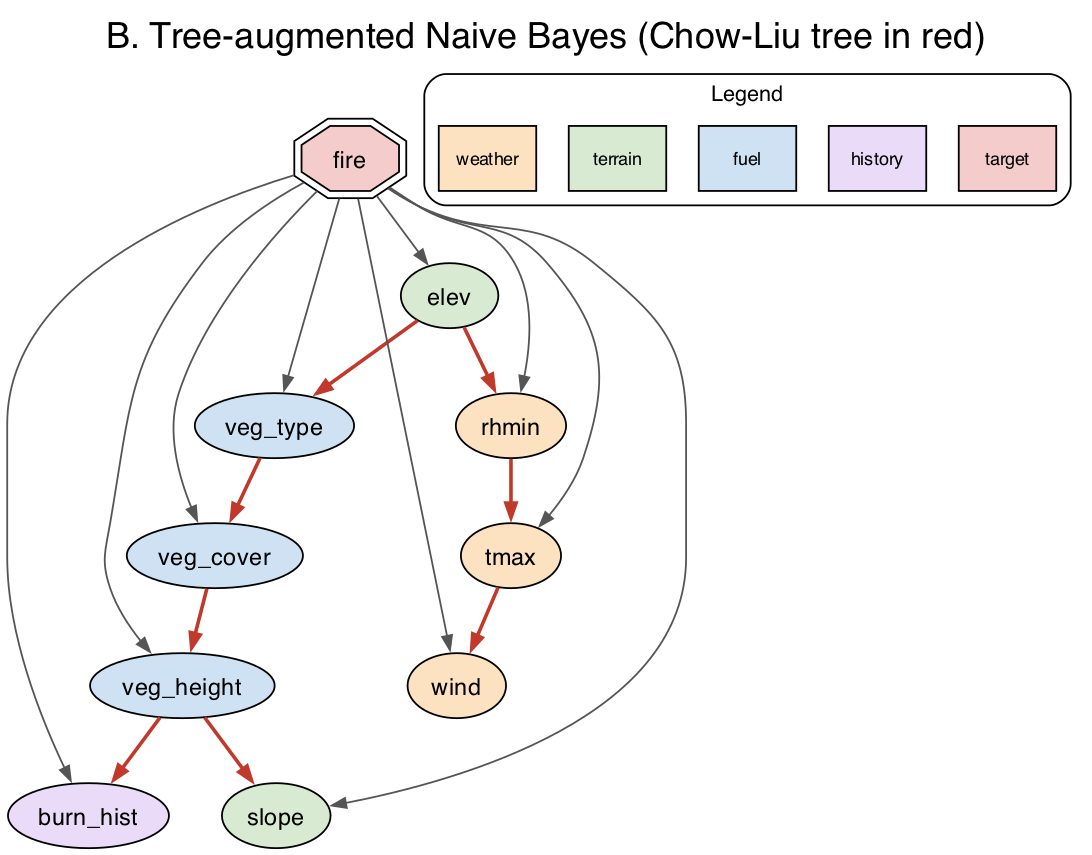
\includegraphics[width=0.32\linewidth]{dag_tan.png}
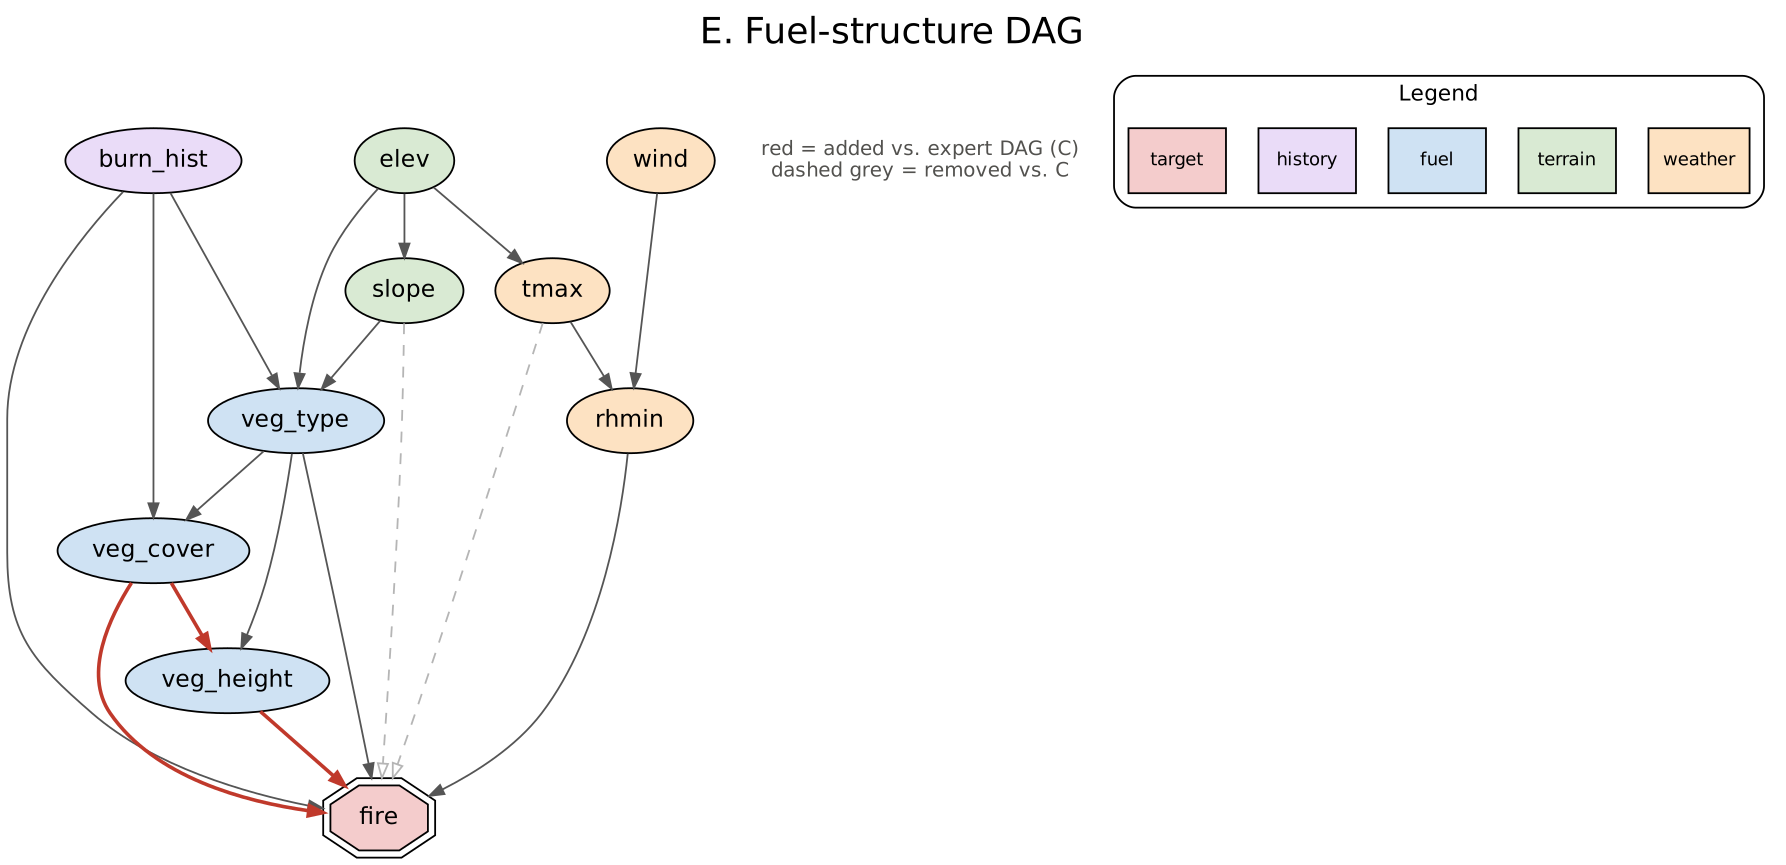
\includegraphics[width=0.32\linewidth]{dag_fuel.png}\\[4pt]
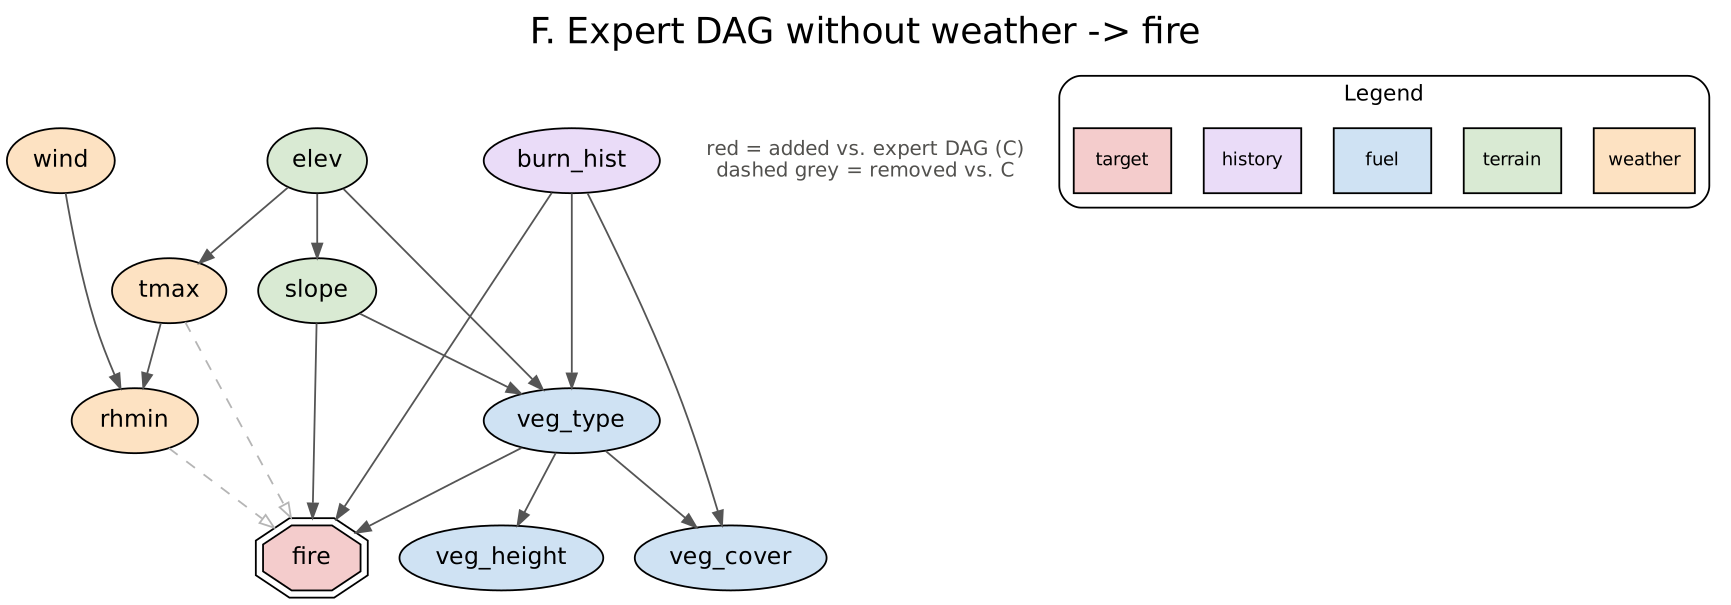
\includegraphics[width=0.32\linewidth]{dag_no_weather.png}
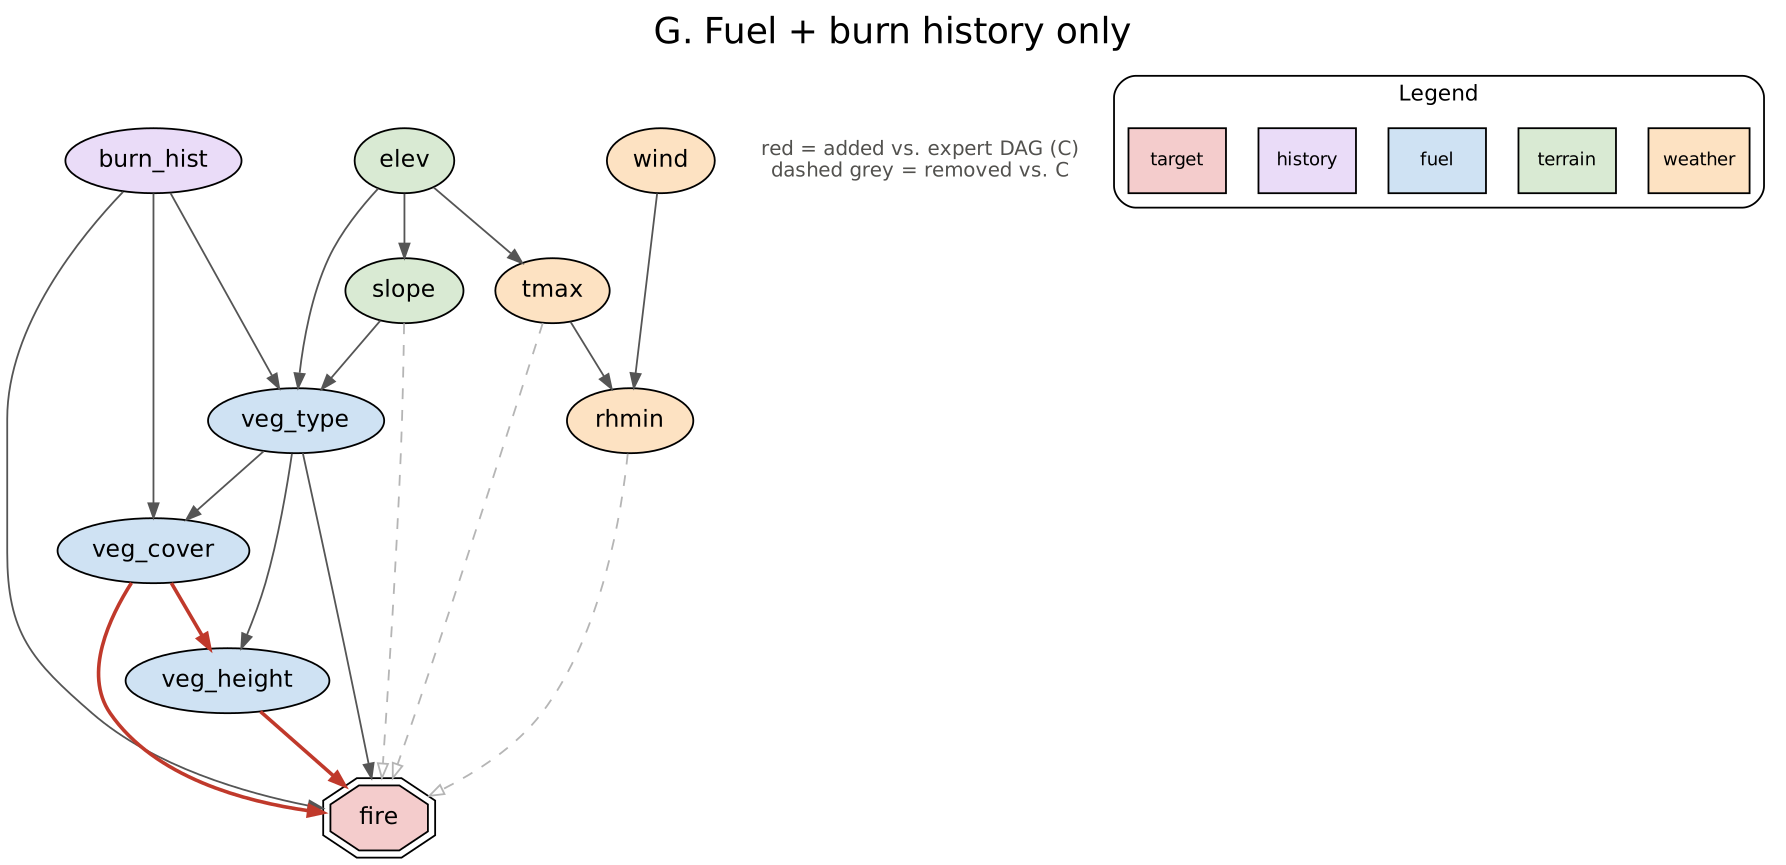
\includegraphics[width=0.32\linewidth]{dag_fuel_only.png}
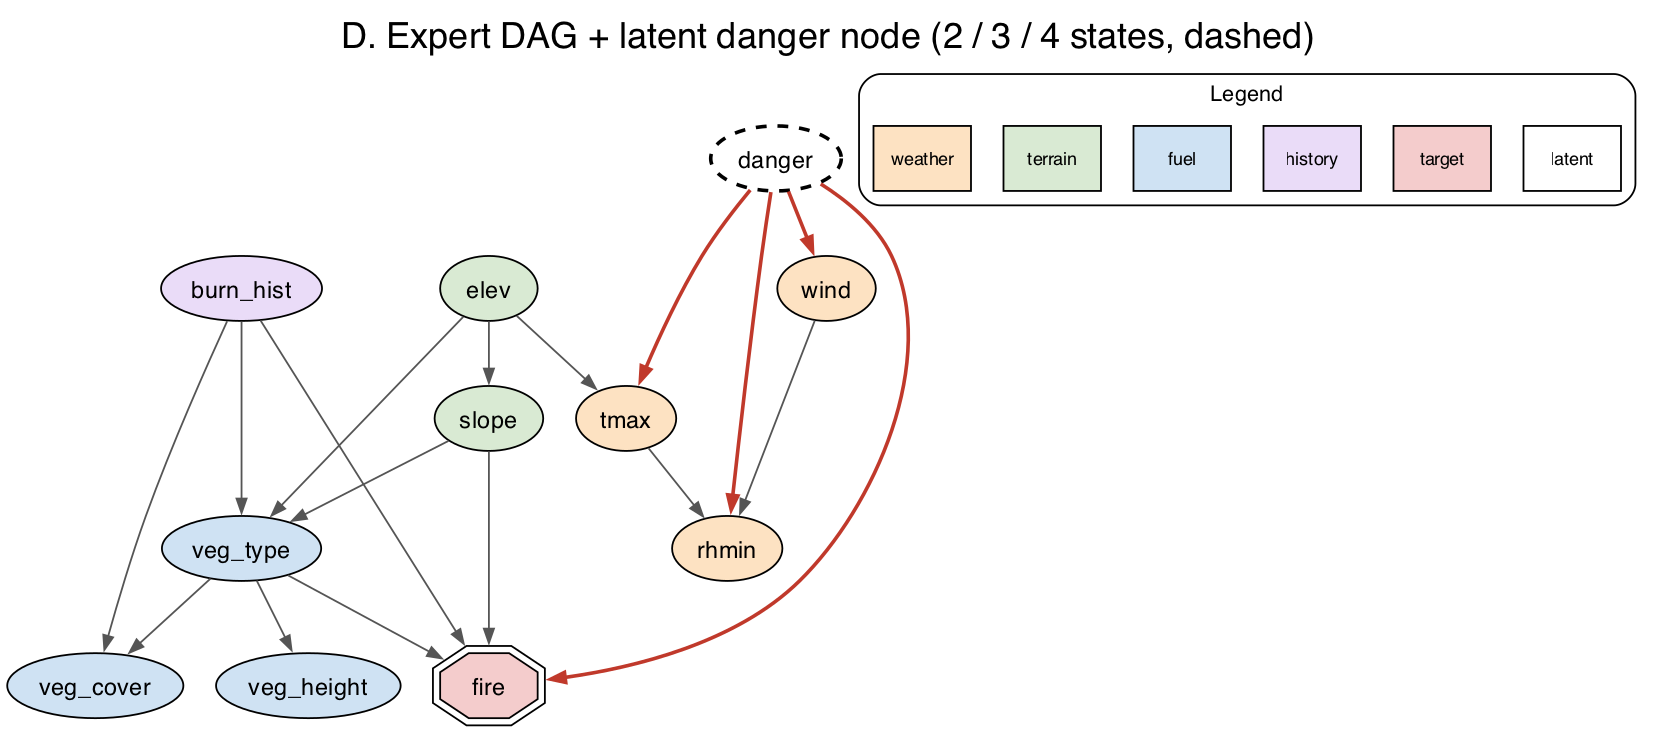
\includegraphics[width=0.32\linewidth]{dag_latent.png}
\caption{Remaining structures: (A) Naive Bayes, (B) TAN with the Chow--Liu tree in red, (E) fuel
structure, (F) no weather and (G) fuel + history only, each drawn against the expert DAG C (red =
edge added, dashed grey = edge removed), and (D) expert DAG with the latent \texttt{danger} node
(dashed, its edges in red).}
\label{fig:dags_app}
\end{figure}

\begin{figure}[htbp]
\centering
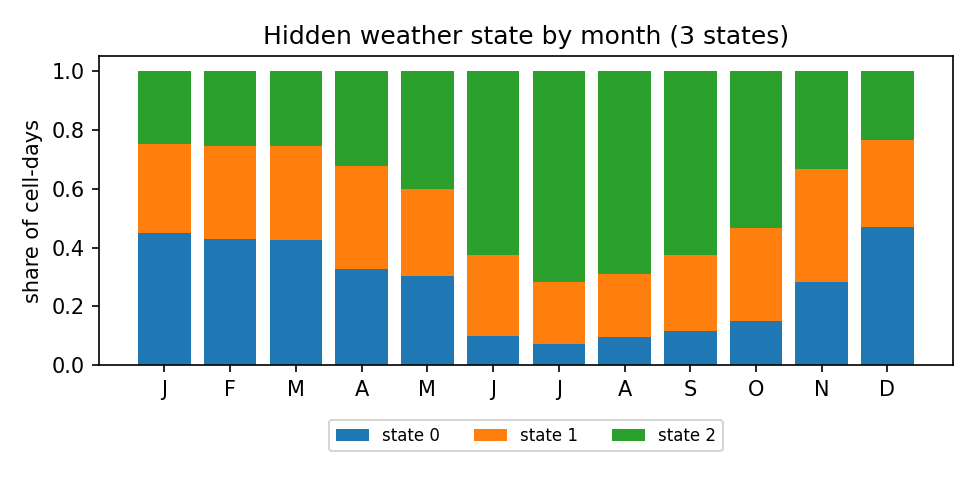
\includegraphics[width=0.6\linewidth]{latent_states_by_month.png}
\caption{Share of cell-days assigned to each hidden state by month (model D, $K=3$, posterior
weighted). State 0: cool/humid/windy; state 1: warm/dry; state 2: hot.}
\label{fig:months}
\end{figure}

\begin{table}[htbp]
\centering
\begin{tabular}{lcccc}
\toprule
Fire history & cool & mild & hot & extreme \\
\midrule
Ignition in last 2 years & 4.5 & 9.2 & 14.7 & 17.0 \\
No fire since 1992 & 0.1 & 0.3 & 0.5 & 0.3 \\
\bottomrule
\end{tabular}
\caption{Fires per 10,000 cell-days in H's fire CPT by temperature, for the two extreme
fire-history states.}
\label{tab:hcpt}
\end{table}

\end{document}
